Le nombre hebdomadaire de consultations lors d'une épidémie de grippe saisonnière, pendant 10 semaines consécutives, est modélisé par la fonction $f$, définie sur l'intervalle $[0 ; 10]$ par :

$f(t)=-25t^{2}+300t+400$ où $t$ représente le nombre de semaines écoulées depuis le début de l'épidémie.

La courbe représentative $\mathcal{C}_{f}$ de la fonction $f$ est donnée ci-dessous dans un repère du plan.

\begin{figure}
	\begin{center}
		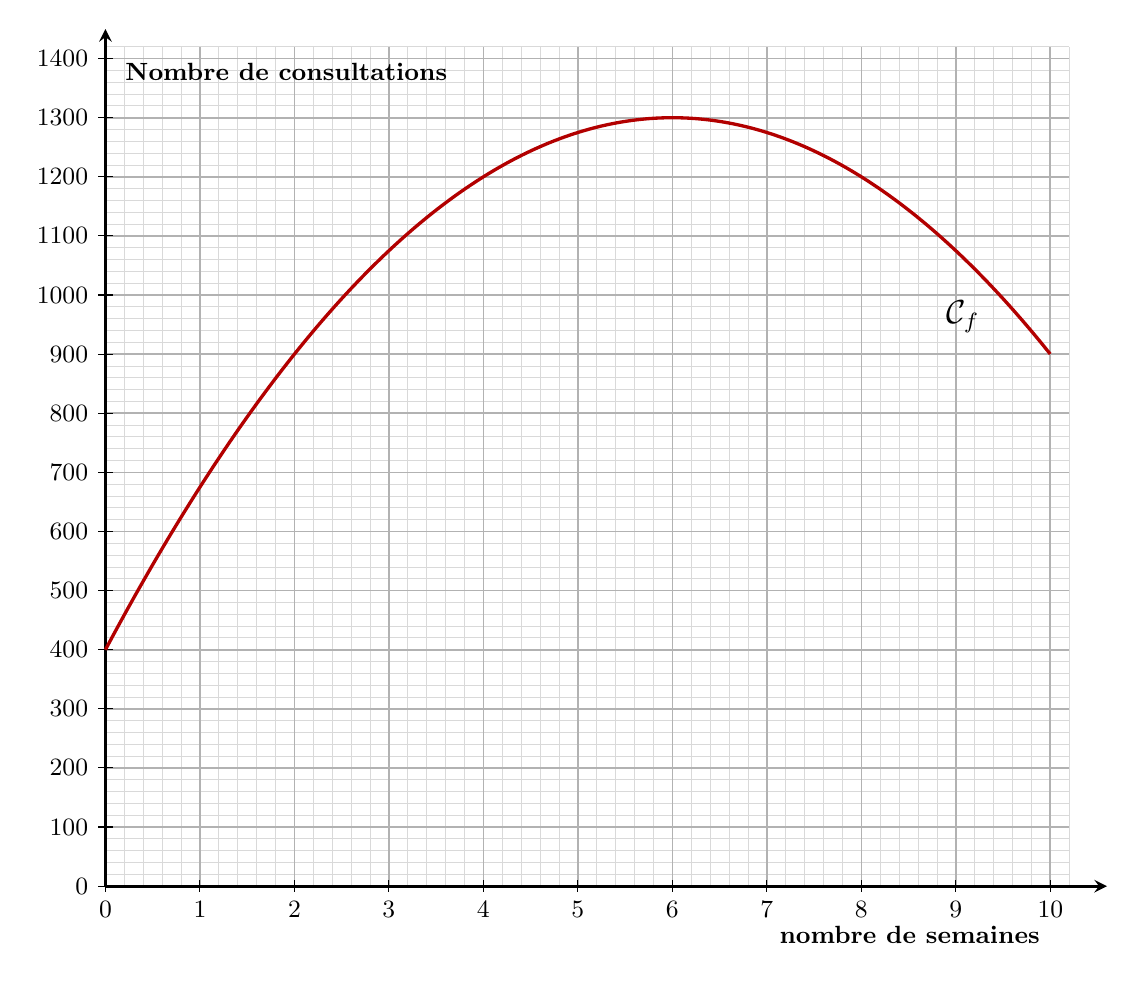
\begin{tikzpicture}[x=1.2cm, y=0.0075cm]
			
			\draw[gray!30, line width=0.3pt] (0,0) grid[xstep=0.2, ystep=20] (10.2,1420);
			
			\draw[gray!60, line width=0.6pt] (0,0) grid[xstep=1, ystep=100] (10.2,1420);

			
			\draw[line width=1pt, ->, >=stealth] (0,0) -- (10.6,0) node[below left, font=\small\bfseries] at (10,-50){nombre de semaines};
			\draw[line width=1pt, ->, >=stealth] (0,0) -- (0,1450) node[below right, font=\small\bfseries] at (0.1,1410){Nombre de consultations};

			
			\foreach \x in {0,1,...,10}
			\draw (\x,10) -- (\x,-10) node[below, font=\small]{$\np{\x}$};

			
			\foreach \y in {0,100,...,1400}
			\draw (0.08,\y) -- (-0.08,\y) node[left, font=\small]{$\np{\y}$};

			
			\draw[red!70!black, line width=1.2pt] plot[smooth, domain=0:10, samples=100] (\x, {-25*\x*\x + 300*\x + 400});
			\node[above right, font=\large] at (8.8, 920) {$\mathcal{C}_f$};
		\end{tikzpicture}
	\end{center}
\end{figure}

\subsection*{Partie A : lecture graphique}

En utilisant le graphique ci-dessus :
\begin{enumerate}
	\item Déterminer le nombre de consultations 2 semaines après le début de l'épidémie.
	\item Déterminer l'intervalle de temps pour lequel le nombre de consultations dépasse \np{1200}.
	\item Au bout de combien de semaines après le début de l'épidémie le nombre de consultations est-il maximal ? Quelle est cette valeur maximale ?
\end{enumerate}

\subsection*{Partie B : Étude de la fonction $f$}

\begin{enumerate}
	\item Calculer $f(0)$. Interpréter le résultat dans le contexte de l'exercice.
	\item Justifier que, pour tout réel $t$ de l'intervalle $[0~;~10]$, $f'(t) = -50t + 300$.
	\item Résoudre dans l'intervalle $[0~;~10]$ l'équation $f'(t)=0$.
	\item Étudier le signe de $f'(t)$, puis dresser le tableau de variation de la fonction $f$ sur l'intervalle $[0~;~10]$. On donne $f(6)=\np{1300}$.
\end{enumerate}
